\documentclass{beamer}
\usepackage{mathrsfs} %Pretty fonts
\usepackage{amsmath}
\usepackage{amssymb}
\usepackage{amsfonts}
\usepackage{amsthm}
\usepackage{bbm}

\newtheorem{proposition}{Proposition}[section]

\mode<presentation>{\usetheme{Madrid}}
%%%% COMMANDS %%%%
\usepackage{xifthen}

% Real Numbers
\newcommand{\RNums}{\mathbb{R}}
% sigma-algebra
\newcommand{\salg}{\sigma\text{-algebra}}
% borel sigma-algebra
\newcommand{\borelsalg}{\mathscr{B}(\RNums)}
% Indicator function
\newcommand{\ind}{\mathbbm{1}}
% F: Sigma Algebra
\newcommand{\salgF}{\mathscr{F}}
% Probability P (P measure)
\newcommand{\Pm}{\mathbb{P}}
% Expectation's E
\newcommand{\E}{\mathbb{E}}
%Expectation with Braces
\newcommand{\Exp}[1]{\E\left[#1\right]}
% Variance
\newcommand{\V}{\mathbb{V}}
%Variance  with Braces
\newcommand{\Var}[1]{\V\left[#1\right]}
% Continuous time stochastic process
\newcommand{\ctspr}{\{X_t\}_{t\geq 0}}
% Discrete time stochastic process
\newcommand{\dtspr}{\{X_n\}_{n\geq 0}}
% Insert only one number in the "align" environment
\newcommand\numberthis{\addtocounter{equation}{1}\tag{\theequation}}
% Measure Space
\newcommand{\MeasureSpace}[1]{(\Omega, \salgF, #1)}
% Proabability Space
\newcommand{\ProbSpace}{\MeasureSpace{\Pm}}
% Norm
\newcommand{\norm}[1]{\left\lVert#1\right\rVert}
% Inner Product
\newcommand{\innerprod}[2]{\langle #1, #2\rangle}
% Family N of processes between a and b
\newcommand{\Nfam}[2]{\mathcal{N}\left[#1, #2\right]}
% Family M of processes between a and b
\newcommand{\Mfam}[2]{\mathcal{M}\left[#1, #2\right]}
%Change of Brownian motion
\newcommand{\DeltaW}[1][]{%
\ifthenelse{\isempty{#1}}{\Delta W_i}{\Delta W_#1}%
}
% differential w.r.t. the brownian motion
\newcommand{\dW}[1][]{%
\ifthenelse{\isempty{#1}}{dW}{dW_#1}%
}
% n-th partial derivative w.r.t. a single variable
\newcommand{\partialwrt}[3][]{
\ifthenelse{\isempty{#1}}
{\frac{\partial #2}{\partial #3}}
{\frac{\partial^{#1} #2}{\partial #3^{#1}}}
}

% Big-oh notation
\newcommand{\bigO}{\mathcal{O}}

% Market
\newcommand{\market}{\{X(t)\}_{t\in[0,T]}}

\title{Theoretical Grounds and Market Adaptations of Financial Fx and Interest Rate Options}
\author{Gerardo Dur\'an Mart\'in}
\institute{Universidad Marista}

\logo{
\includegraphics[height=1.7cm]{UMA_logo}}

\begin{document}
%Generates the title page
\frame{\titlepage}

\AtBeginSection[]{
\begin{frame}
	\frametitle{Table of Contents}
	\tableofcontents[currentsection]
\end{frame}
}

\section{Financial Markets}

%% Market Assumptions
\begin{frame}
\frametitle{Some Important Definitions}

\only<1->{
\begin{definition}[Security]
	A security is an instrument that either represents ownership or that derives its value from a commodity.
\end{definition}
}

\only<2->{
\begin{definition}[Market]
	A market is the place where buyers meet sellers to exchange securities.
\end{definition}
}

\only<3->{
\begin{definition}[Arbitrage]
	We define an arbitrage as the probability of making a risk-free profit from a suitable market strategy.
	$$
		\Pm{(\text{Risk-free profit} > 0)} = 1
	$$
\end{definition}
}
\end{frame}


\begin{frame}
\frametitle{Market Assumptions}
\begin{itemize}
	\item Many buyers and sellers (liquidity);
	\item possible to lend and borrow at the same rate interest rate $r$;
	\item Market participants take advantage of arbitrage opportunity, thereby correcting any deviation from the actual value of any asset.
	\item All participants have the same information.
\end{itemize}
\end{frame}

%% Instruments
\begin{frame}
\frametitle{The Instruments}
	
	\begin{columns}[c]	
	
	\column{0.45\textwidth}
	\begin{itemize}
		\item <1-| alert@1> Bonds
		\item <2-| alert@2> Stocks
		\item <3-| alert@3> Foreign Exchange Currencies
		\item <4-| alert@4> Derivatives
	\end{itemize}
	
	\column{0.5\textwidth}
	\only<1>{
	A Bond is a debt obligation, its main function is to raise capital for the issuer of the bond. In turn, the buyer of the bond receives interest on the amount loaned.
	}
	\only<2>{
	A stock is a security that represents ownership on a fraction of a corporation. The return on the company for the owner of a stock is represented as a dividend.
	}
	\only<3>{
	``One country’s currency freely convertible in the foreign exchange market.'' (Kozikowski, 2013)
	}
	\only<4>{
	``[A derivative is] a financial instrument whose value depends on (or derives from) the values of other, more basic, underlying variables.'' (Hull, 2014)
	}
	\end{columns}
\end{frame}

%%Forwards
\begin{frame}
\frametitle{Derivatives: An Example}

	\begin{definition}[Forward]
		A forward is a derivative contract that gives the buyer both the right, and the obligation to to purchase a specified amount of the stock at some future time $T$, at a price $K$. The value of the forward today is 0.
	\end{definition}
	The payoff of the forward is $S_T - K$. What is the $K$ such that the contract has zero value today and has no possibility of arbitrage?
	
	\begin{figure}
	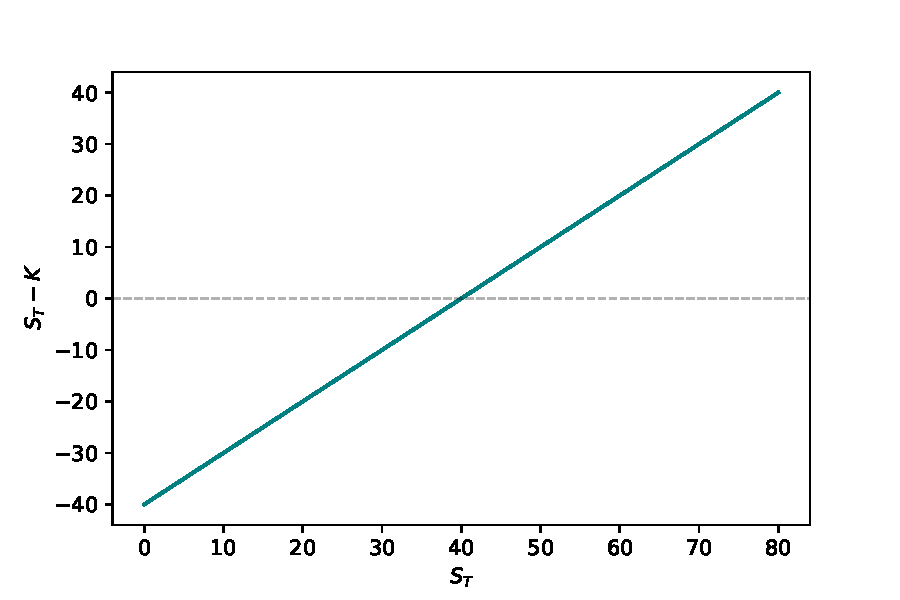
\includegraphics[width=0.45\textwidth]{../images/foward_payoff}
	\end{figure}
\end{frame}

\begin{frame}
\frametitle{Derivatives: An Example (cont'd)}
Assume a continuously compounded interest rate $r$, denote $S_t$ the value of the stock at time $t$. At $t=T$ the value of the forward is
$$
	S_T - K = 0
$$

By no arbitrage, the present value of the strategy is
$$
	S_0 - Ke^{-rT} = 0 \implies K = S_0e^{rT}
$$
Therefore, $S_0e^{rT}$ is the the value that guarantees no arbitrage.
\end{frame}

\begin{frame}
\frametitle{Derivatives: An Example (cont'd)}

(Why?)

Assume $K^\prime > K = S_0e^{rT}$. 
\begin{itemize}
	\item At $t=0$, borrow $S_0$; purchase the stock; and take a short position the forward contract.
	\item At $t=T$, receive $K^\prime$; give the forward; and repay $S_0e^{rT}$. Profit $K^\prime - S_0e^{rT}$.
\end{itemize}

The same can be said for $K^\prime < K$, by taking a long position.
\end{frame}

%%Option Pricing
\begin{frame}
\frametitle{Derivatives: Another Example}

\begin{definition}[European Call Option]
A European call option is a derivative contract that gives the buyer the right, but not the obligation to purchase a specified amount of stock at some future time $T$, at a price $K$.
\end{definition}

The payoff of the option is $\max\{S_T - K, 0\}$. What is the price of the option today that guarantees no arbitrage?

\begin{figure}
	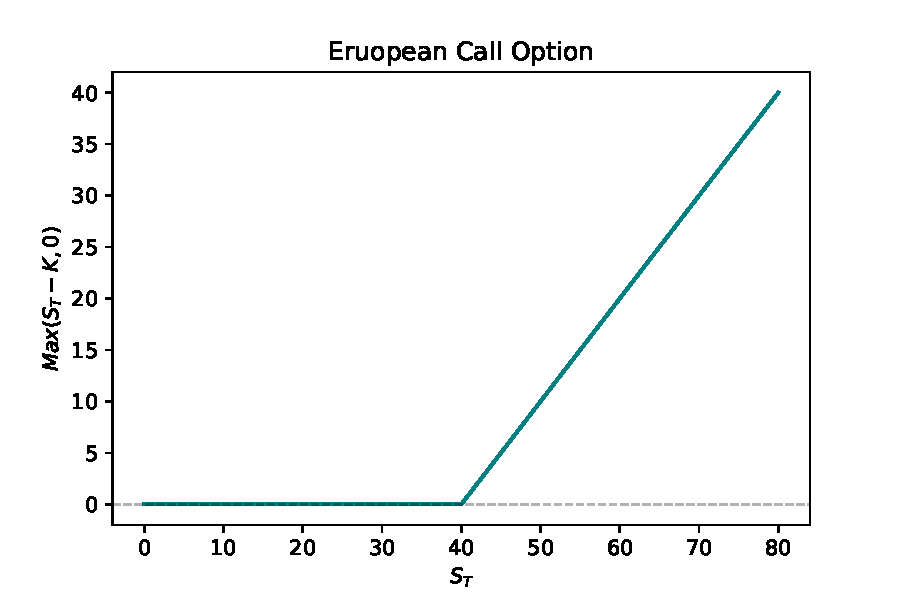
\includegraphics[width=0.45\textwidth=]{../images/Call}
\end{figure}
\end{frame}

\section{Probability and Measure Theory}
\begin{frame}
\frametitle{Measures and $\salg$s}
\begin{definition}[$\salg$]
	Let $\Omega$ a set of points $\omega$. $\salgF$ is a $\salg$ if
	\begin{enumerate}
		\item $\Omega \in \salgF$;
		\item if $A \in 	\salgF$, then $A^c \in \salgF$; and
		\item if $\{A_n\}_{n\geq 1} \in \salgF$, then $\bigcup_n A_n \in \salgF$.
	\end{enumerate}
\end{definition}

\begin{definition}
	Let $\emptyset \neq A\subseteq\Omega$, we define the $\salg$ generated by $A$ as
	\[
		\sigma(A) := \bigcap\{\salgF | \salgF \text{ is a $\salg$ and } A \subseteq \salgF\}
	\]
\end{definition}
\end{frame}


\begin{frame}
\frametitle{Probability Theory}
\begin{definition}[Measurable Space]
An ordered tripe $\ProbSpace$ where
\begin{itemize}
	\item $\Omega$ is a set of points $\omega$;
	\item $\salgF$ is a $\salg$ of elements of $\Omega$; and
	\item $\Pm$ is a probability on $\salgF$. 
\end{itemize}
\end{definition}

\begin{definition}[Random Variable]
	\[
		X^{-1}(B) = \{\omega \in \Omega | X(\omega) \in B\} \ \forall \ B \subseteq \borelsalg.
	\]
\end{definition}
\end{frame}

%% Integrals
\begin{frame}
\frametitle{Integrals}

\only<1>{
\begin{definition}[Integral v.1]
	Let $\MeasureSpace{\mu}$ be a measure space, we define the Lebesgue integral (or integral)of the indicator function $\ind_A$ w.r.t. $\mu$ as
	\[
		\int_\Omega \ind_A d\mu := \mu(A)
	\]
\end{definition}
}

\only<2>{
\begin{definition}[Simple Function]
	Let $(\Omega, \salgF)$ a measurable space and $X$ an $\salgF$-measurable function. It is said that $X$ is a \textbf{simple function} if it takes only a unique finite number of values $\{x_i\}_{i=1}^{n} \in \RNums$ over measurable sets $\{A_i\}$. Then, $X$ can be written as
	\[
		X(\omega) = \sum_{i=1}^{n}x_i\ind_{A_i}
	\]
\end{definition}

\begin{definition}[Integral v.2]
	let $X$ be a simple function, we define the integral of $X$ w.r.t. $\mu$ as:
	\[
		\int_\Omega X(\omega) d\mu(\omega) := \sum_{i=1}^{n}x_i\mu(A_i)
	\]
\end{definition}
}

\only<3>{
\begin{definition}[Integral v.3]
For any nonnegative function $X$, we define the integral of $X$ w.r.t. a measure $\mu$ as
\[
	\int_\Omega Xd\mu := \sup\left\{\int_\Omega h d\mu \ | \ 0 \leq h \leq X \text{, $h$ is simple}\right\}
\]
\end{definition}
\begin{figure}
	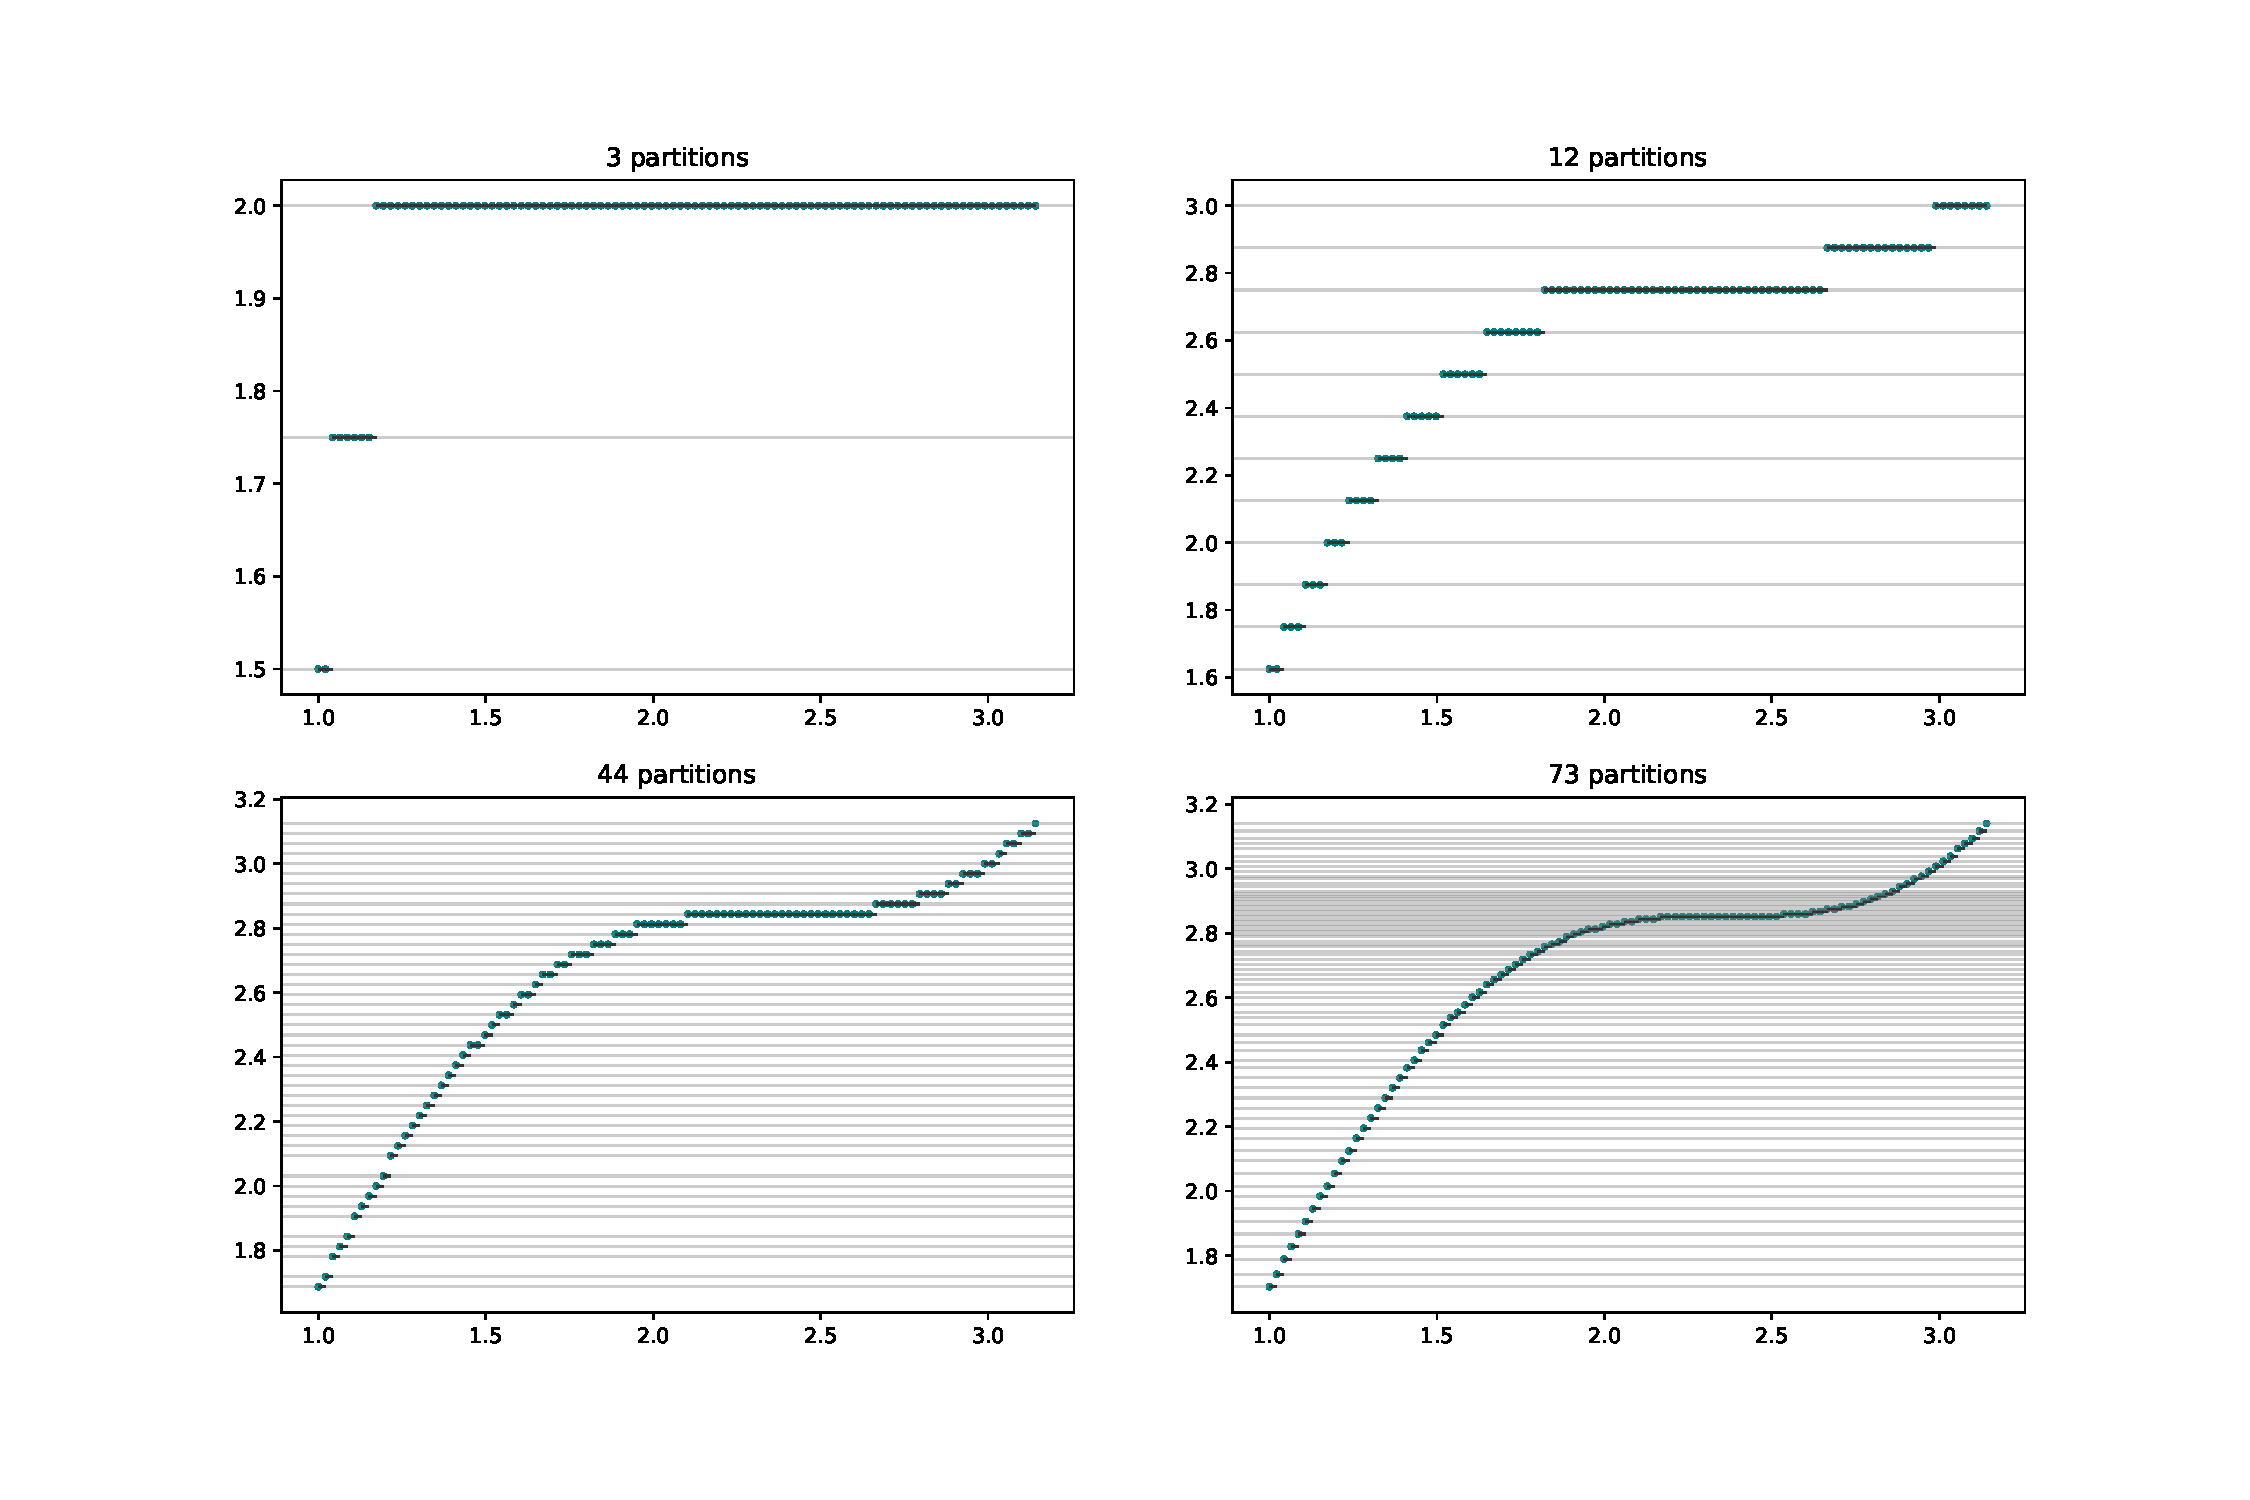
\includegraphics[width=0.50\textwidth]{../images/simple_sine}
\end{figure}
}
\end{frame}

\begin{frame}
\begin{proposition}
	For any $X$, $Y$ $\salgF$-measurable functions in $L_1$; $A$, $B$ members of $\salgF$:
	\[
		X \geq 0 \implies \int_\Omega X d\mu \geq 0
	\]
	
	If $X \leq Y$ (monotonicity),
	\[
		\int_\Omega X d\mu \leq \int_\Omega Y d\mu
	\]
	
	If $A \subseteq B$ and $X \geq 0$,
	\[
		\int_A X d\mu \leq \int_B X d\mu
	\]
	
	If $\alpha$, $\beta$ $\in \RNums$ (linearity),
	\[
	\int_\Omega (\alpha X + \beta Y) d\mu = \alpha \int_\Omega X d\mu + \beta \int_\Omega Y d\mu
	\]
\end{proposition}
\end{frame}

\begin{frame}
\begin{theorem}[\textbf{Radon Nikodym Theorem}]\label{th:radon-nikodym}
Let $\mu$ and $\lambda$ be $\sigma$-finite positive measures defined on $(\Omega, \mathscr{F})$ such that, for every $A \in \mathscr{F}$, $\lambda(A) = 0 \implies \mu(A)= 0$. Then, there exists a function $f: \Omega \to [0, \infty]$ such that
\[
	\mu(A) = \int_A f d\lambda.
\]

Where the function $f$ is defined up to sets with measure zero. $f$ is sometimes called the Radon-Nikodym derivative and it can be written as $\frac{d\mu}{d\lambda}$
\end{theorem}

\end{frame}

%% Expectation
\begin{frame}
\frametitle{Expectation}
	\begin{definition}
		Let $X$ be a r.v. on $\ProbSpace$, we define the expectation of $X$ with respect to (w.r.t.) $\Pm$ as
		\[
			\E[X] := \int_\Omega X(\omega) d\Pm(\omega)
		\]
	\end{definition}
	
	\begin{definition}[Conditional Expectation w.r.t. a $\sigma$-algebra]
The conditional expectation of a nonnegative random variable $X$ with respect to the $\sigma$-algebra $\mathscr{G}$ is a nonnegative random variable denoted $\mathbb{E}[X | \mathscr{G}]$ or $\mathbb{E}[X | \mathscr{G}](\omega)$ such that,
\begin{enumerate}
	\item $\mathbb{E}[X | \mathscr{G}]$ is $\mathscr{G}$-measurable; and
	\item For every $A \in \mathscr{G}$,
	\[\int_A X d\Pm = \int_A \mathbb{E}[X | \mathscr{G}] d\Pm\].
\end{enumerate}
\end{definition}
\end{frame}

\begin{frame}
\begin{proposition}
	\begin{enumerate}
		\item If $a, b \in \RNums$, $\E[\alpha X + \beta Y | \mathscr{G}]$ = $\alpha \E[X | \mathscr{G}] + \beta\E[Y | \mathscr{G}]$;
		\item $\E[\E[X | \salgF]] = \E[X]$;
		\item $\E[\E[X | \salgF_2] | \salgF_1]$ = $[X | \salgF_1]$ if $\salgF_1 \subseteq \salgF_2$;
		\item $\E[\E[X | \salgF_2] | \salgF_1]$ = $[X | \salgF_2]$ if $\salgF_2 \subseteq \salgF_1$; and
		\item Let $X$ be a random variable such that $X \perp \mathscr{G}$ then, $\E[X|\mathscr{G}] = \E[X]$. Consequently, for any borel-measurable function $h$, $\E[h(X)|\mathscr{G}] = \E[h(X)]$.
	\end{enumerate}
\end{proposition}
\end{frame}
\end{document}